\documentclass[11pt]{article}

    \usepackage[breakable]{tcolorbox}
    \usepackage{parskip} % Stop auto-indenting (to mimic markdown behaviour)
    
    \usepackage{iftex}
    \ifPDFTeX
    	\usepackage[T1]{fontenc}
    	\usepackage{mathpazo}
    \else
    	\usepackage{fontspec}
    \fi

    % Basic figure setup, for now with no caption control since it's done
    % automatically by Pandoc (which extracts ![](path) syntax from Markdown).
    \usepackage{graphicx}
    % Maintain compatibility with old templates. Remove in nbconvert 6.0
    \let\Oldincludegraphics\includegraphics
    % Ensure that by default, figures have no caption (until we provide a
    % proper Figure object with a Caption API and a way to capture that
    % in the conversion process - todo).
    \usepackage{caption}
    \DeclareCaptionFormat{nocaption}{}
    \captionsetup{format=nocaption,aboveskip=0pt,belowskip=0pt}

    \usepackage[Export]{adjustbox} % Used to constrain images to a maximum size
    \adjustboxset{max size={0.9\linewidth}{0.9\paperheight}}
    \usepackage{float}
    \floatplacement{figure}{H} % forces figures to be placed at the correct location
    \usepackage{xcolor} % Allow colors to be defined
    \usepackage{enumerate} % Needed for markdown enumerations to work
    \usepackage{geometry} % Used to adjust the document margins
    \usepackage{amsmath} % Equations
    \usepackage{amssymb} % Equations
    \usepackage{textcomp} % defines textquotesingle
    % Hack from http://tex.stackexchange.com/a/47451/13684:
    \AtBeginDocument{%
        \def\PYZsq{\textquotesingle}% Upright quotes in Pygmentized code
    }
    \usepackage{upquote} % Upright quotes for verbatim code
    \usepackage{eurosym} % defines \euro
    \usepackage[mathletters]{ucs} % Extended unicode (utf-8) support
    \usepackage{fancyvrb} % verbatim replacement that allows latex
    \usepackage{grffile} % extends the file name processing of package graphics 
                         % to support a larger range
    \makeatletter % fix for grffile with XeLaTeX
    \def\Gread@@xetex#1{%
      \IfFileExists{"\Gin@base".bb}%
      {\Gread@eps{\Gin@base.bb}}%
      {\Gread@@xetex@aux#1}%
    }
    \makeatother

    % The hyperref package gives us a pdf with properly built
    % internal navigation ('pdf bookmarks' for the table of contents,
    % internal cross-reference links, web links for URLs, etc.)
    \usepackage{hyperref}
    % The default LaTeX title has an obnoxious amount of whitespace. By default,
    % titling removes some of it. It also provides customization options.
    \usepackage{titling}
    \usepackage{longtable} % longtable support required by pandoc >1.10
    \usepackage{booktabs}  % table support for pandoc > 1.12.2
    \usepackage[inline]{enumitem} % IRkernel/repr support (it uses the enumerate* environment)
    \usepackage[normalem]{ulem} % ulem is needed to support strikethroughs (\sout)
                                % normalem makes italics be italics, not underlines
    \usepackage{mathrsfs}
    

    
    % Colors for the hyperref package
    \definecolor{urlcolor}{rgb}{0,.145,.698}
    \definecolor{linkcolor}{rgb}{.71,0.21,0.01}
    \definecolor{citecolor}{rgb}{.12,.54,.11}

    % ANSI colors
    \definecolor{ansi-black}{HTML}{3E424D}
    \definecolor{ansi-black-intense}{HTML}{282C36}
    \definecolor{ansi-red}{HTML}{E75C58}
    \definecolor{ansi-red-intense}{HTML}{B22B31}
    \definecolor{ansi-green}{HTML}{00A250}
    \definecolor{ansi-green-intense}{HTML}{007427}
    \definecolor{ansi-yellow}{HTML}{DDB62B}
    \definecolor{ansi-yellow-intense}{HTML}{B27D12}
    \definecolor{ansi-blue}{HTML}{208FFB}
    \definecolor{ansi-blue-intense}{HTML}{0065CA}
    \definecolor{ansi-magenta}{HTML}{D160C4}
    \definecolor{ansi-magenta-intense}{HTML}{A03196}
    \definecolor{ansi-cyan}{HTML}{60C6C8}
    \definecolor{ansi-cyan-intense}{HTML}{258F8F}
    \definecolor{ansi-white}{HTML}{C5C1B4}
    \definecolor{ansi-white-intense}{HTML}{A1A6B2}
    \definecolor{ansi-default-inverse-fg}{HTML}{FFFFFF}
    \definecolor{ansi-default-inverse-bg}{HTML}{000000}

    % commands and environments needed by pandoc snippets
    % extracted from the output of `pandoc -s`
    \providecommand{\tightlist}{%
      \setlength{\itemsep}{0pt}\setlength{\parskip}{0pt}}
    \DefineVerbatimEnvironment{Highlighting}{Verbatim}{commandchars=\\\{\}}
    % Add ',fontsize=\small' for more characters per line
    \newenvironment{Shaded}{}{}
    \newcommand{\KeywordTok}[1]{\textcolor[rgb]{0.00,0.44,0.13}{\textbf{{#1}}}}
    \newcommand{\DataTypeTok}[1]{\textcolor[rgb]{0.56,0.13,0.00}{{#1}}}
    \newcommand{\DecValTok}[1]{\textcolor[rgb]{0.25,0.63,0.44}{{#1}}}
    \newcommand{\BaseNTok}[1]{\textcolor[rgb]{0.25,0.63,0.44}{{#1}}}
    \newcommand{\FloatTok}[1]{\textcolor[rgb]{0.25,0.63,0.44}{{#1}}}
    \newcommand{\CharTok}[1]{\textcolor[rgb]{0.25,0.44,0.63}{{#1}}}
    \newcommand{\StringTok}[1]{\textcolor[rgb]{0.25,0.44,0.63}{{#1}}}
    \newcommand{\CommentTok}[1]{\textcolor[rgb]{0.38,0.63,0.69}{\textit{{#1}}}}
    \newcommand{\OtherTok}[1]{\textcolor[rgb]{0.00,0.44,0.13}{{#1}}}
    \newcommand{\AlertTok}[1]{\textcolor[rgb]{1.00,0.00,0.00}{\textbf{{#1}}}}
    \newcommand{\FunctionTok}[1]{\textcolor[rgb]{0.02,0.16,0.49}{{#1}}}
    \newcommand{\RegionMarkerTok}[1]{{#1}}
    \newcommand{\ErrorTok}[1]{\textcolor[rgb]{1.00,0.00,0.00}{\textbf{{#1}}}}
    \newcommand{\NormalTok}[1]{{#1}}
    
    % Additional commands for more recent versions of Pandoc
    \newcommand{\ConstantTok}[1]{\textcolor[rgb]{0.53,0.00,0.00}{{#1}}}
    \newcommand{\SpecialCharTok}[1]{\textcolor[rgb]{0.25,0.44,0.63}{{#1}}}
    \newcommand{\VerbatimStringTok}[1]{\textcolor[rgb]{0.25,0.44,0.63}{{#1}}}
    \newcommand{\SpecialStringTok}[1]{\textcolor[rgb]{0.73,0.40,0.53}{{#1}}}
    \newcommand{\ImportTok}[1]{{#1}}
    \newcommand{\DocumentationTok}[1]{\textcolor[rgb]{0.73,0.13,0.13}{\textit{{#1}}}}
    \newcommand{\AnnotationTok}[1]{\textcolor[rgb]{0.38,0.63,0.69}{\textbf{\textit{{#1}}}}}
    \newcommand{\CommentVarTok}[1]{\textcolor[rgb]{0.38,0.63,0.69}{\textbf{\textit{{#1}}}}}
    \newcommand{\VariableTok}[1]{\textcolor[rgb]{0.10,0.09,0.49}{{#1}}}
    \newcommand{\ControlFlowTok}[1]{\textcolor[rgb]{0.00,0.44,0.13}{\textbf{{#1}}}}
    \newcommand{\OperatorTok}[1]{\textcolor[rgb]{0.40,0.40,0.40}{{#1}}}
    \newcommand{\BuiltInTok}[1]{{#1}}
    \newcommand{\ExtensionTok}[1]{{#1}}
    \newcommand{\PreprocessorTok}[1]{\textcolor[rgb]{0.74,0.48,0.00}{{#1}}}
    \newcommand{\AttributeTok}[1]{\textcolor[rgb]{0.49,0.56,0.16}{{#1}}}
    \newcommand{\InformationTok}[1]{\textcolor[rgb]{0.38,0.63,0.69}{\textbf{\textit{{#1}}}}}
    \newcommand{\WarningTok}[1]{\textcolor[rgb]{0.38,0.63,0.69}{\textbf{\textit{{#1}}}}}
    
    
    % Define a nice break command that doesn't care if a line doesn't already
    % exist.
    \def\br{\hspace*{\fill} \\* }
    % Math Jax compatibility definitions
    \def\gt{>}
    \def\lt{<}
    \let\Oldtex\TeX
    \let\Oldlatex\LaTeX
    \renewcommand{\TeX}{\textrm{\Oldtex}}
    \renewcommand{\LaTeX}{\textrm{\Oldlatex}}
    % Document parameters
    % Document title
    \title{README}
    
    
    
    
    
% Pygments definitions
\makeatletter
\def\PY@reset{\let\PY@it=\relax \let\PY@bf=\relax%
    \let\PY@ul=\relax \let\PY@tc=\relax%
    \let\PY@bc=\relax \let\PY@ff=\relax}
\def\PY@tok#1{\csname PY@tok@#1\endcsname}
\def\PY@toks#1+{\ifx\relax#1\empty\else%
    \PY@tok{#1}\expandafter\PY@toks\fi}
\def\PY@do#1{\PY@bc{\PY@tc{\PY@ul{%
    \PY@it{\PY@bf{\PY@ff{#1}}}}}}}
\def\PY#1#2{\PY@reset\PY@toks#1+\relax+\PY@do{#2}}

\expandafter\def\csname PY@tok@w\endcsname{\def\PY@tc##1{\textcolor[rgb]{0.73,0.73,0.73}{##1}}}
\expandafter\def\csname PY@tok@c\endcsname{\let\PY@it=\textit\def\PY@tc##1{\textcolor[rgb]{0.25,0.50,0.50}{##1}}}
\expandafter\def\csname PY@tok@cp\endcsname{\def\PY@tc##1{\textcolor[rgb]{0.74,0.48,0.00}{##1}}}
\expandafter\def\csname PY@tok@k\endcsname{\let\PY@bf=\textbf\def\PY@tc##1{\textcolor[rgb]{0.00,0.50,0.00}{##1}}}
\expandafter\def\csname PY@tok@kp\endcsname{\def\PY@tc##1{\textcolor[rgb]{0.00,0.50,0.00}{##1}}}
\expandafter\def\csname PY@tok@kt\endcsname{\def\PY@tc##1{\textcolor[rgb]{0.69,0.00,0.25}{##1}}}
\expandafter\def\csname PY@tok@o\endcsname{\def\PY@tc##1{\textcolor[rgb]{0.40,0.40,0.40}{##1}}}
\expandafter\def\csname PY@tok@ow\endcsname{\let\PY@bf=\textbf\def\PY@tc##1{\textcolor[rgb]{0.67,0.13,1.00}{##1}}}
\expandafter\def\csname PY@tok@nb\endcsname{\def\PY@tc##1{\textcolor[rgb]{0.00,0.50,0.00}{##1}}}
\expandafter\def\csname PY@tok@nf\endcsname{\def\PY@tc##1{\textcolor[rgb]{0.00,0.00,1.00}{##1}}}
\expandafter\def\csname PY@tok@nc\endcsname{\let\PY@bf=\textbf\def\PY@tc##1{\textcolor[rgb]{0.00,0.00,1.00}{##1}}}
\expandafter\def\csname PY@tok@nn\endcsname{\let\PY@bf=\textbf\def\PY@tc##1{\textcolor[rgb]{0.00,0.00,1.00}{##1}}}
\expandafter\def\csname PY@tok@ne\endcsname{\let\PY@bf=\textbf\def\PY@tc##1{\textcolor[rgb]{0.82,0.25,0.23}{##1}}}
\expandafter\def\csname PY@tok@nv\endcsname{\def\PY@tc##1{\textcolor[rgb]{0.10,0.09,0.49}{##1}}}
\expandafter\def\csname PY@tok@no\endcsname{\def\PY@tc##1{\textcolor[rgb]{0.53,0.00,0.00}{##1}}}
\expandafter\def\csname PY@tok@nl\endcsname{\def\PY@tc##1{\textcolor[rgb]{0.63,0.63,0.00}{##1}}}
\expandafter\def\csname PY@tok@ni\endcsname{\let\PY@bf=\textbf\def\PY@tc##1{\textcolor[rgb]{0.60,0.60,0.60}{##1}}}
\expandafter\def\csname PY@tok@na\endcsname{\def\PY@tc##1{\textcolor[rgb]{0.49,0.56,0.16}{##1}}}
\expandafter\def\csname PY@tok@nt\endcsname{\let\PY@bf=\textbf\def\PY@tc##1{\textcolor[rgb]{0.00,0.50,0.00}{##1}}}
\expandafter\def\csname PY@tok@nd\endcsname{\def\PY@tc##1{\textcolor[rgb]{0.67,0.13,1.00}{##1}}}
\expandafter\def\csname PY@tok@s\endcsname{\def\PY@tc##1{\textcolor[rgb]{0.73,0.13,0.13}{##1}}}
\expandafter\def\csname PY@tok@sd\endcsname{\let\PY@it=\textit\def\PY@tc##1{\textcolor[rgb]{0.73,0.13,0.13}{##1}}}
\expandafter\def\csname PY@tok@si\endcsname{\let\PY@bf=\textbf\def\PY@tc##1{\textcolor[rgb]{0.73,0.40,0.53}{##1}}}
\expandafter\def\csname PY@tok@se\endcsname{\let\PY@bf=\textbf\def\PY@tc##1{\textcolor[rgb]{0.73,0.40,0.13}{##1}}}
\expandafter\def\csname PY@tok@sr\endcsname{\def\PY@tc##1{\textcolor[rgb]{0.73,0.40,0.53}{##1}}}
\expandafter\def\csname PY@tok@ss\endcsname{\def\PY@tc##1{\textcolor[rgb]{0.10,0.09,0.49}{##1}}}
\expandafter\def\csname PY@tok@sx\endcsname{\def\PY@tc##1{\textcolor[rgb]{0.00,0.50,0.00}{##1}}}
\expandafter\def\csname PY@tok@m\endcsname{\def\PY@tc##1{\textcolor[rgb]{0.40,0.40,0.40}{##1}}}
\expandafter\def\csname PY@tok@gh\endcsname{\let\PY@bf=\textbf\def\PY@tc##1{\textcolor[rgb]{0.00,0.00,0.50}{##1}}}
\expandafter\def\csname PY@tok@gu\endcsname{\let\PY@bf=\textbf\def\PY@tc##1{\textcolor[rgb]{0.50,0.00,0.50}{##1}}}
\expandafter\def\csname PY@tok@gd\endcsname{\def\PY@tc##1{\textcolor[rgb]{0.63,0.00,0.00}{##1}}}
\expandafter\def\csname PY@tok@gi\endcsname{\def\PY@tc##1{\textcolor[rgb]{0.00,0.63,0.00}{##1}}}
\expandafter\def\csname PY@tok@gr\endcsname{\def\PY@tc##1{\textcolor[rgb]{1.00,0.00,0.00}{##1}}}
\expandafter\def\csname PY@tok@ge\endcsname{\let\PY@it=\textit}
\expandafter\def\csname PY@tok@gs\endcsname{\let\PY@bf=\textbf}
\expandafter\def\csname PY@tok@gp\endcsname{\let\PY@bf=\textbf\def\PY@tc##1{\textcolor[rgb]{0.00,0.00,0.50}{##1}}}
\expandafter\def\csname PY@tok@go\endcsname{\def\PY@tc##1{\textcolor[rgb]{0.53,0.53,0.53}{##1}}}
\expandafter\def\csname PY@tok@gt\endcsname{\def\PY@tc##1{\textcolor[rgb]{0.00,0.27,0.87}{##1}}}
\expandafter\def\csname PY@tok@err\endcsname{\def\PY@bc##1{\setlength{\fboxsep}{0pt}\fcolorbox[rgb]{1.00,0.00,0.00}{1,1,1}{\strut ##1}}}
\expandafter\def\csname PY@tok@kc\endcsname{\let\PY@bf=\textbf\def\PY@tc##1{\textcolor[rgb]{0.00,0.50,0.00}{##1}}}
\expandafter\def\csname PY@tok@kd\endcsname{\let\PY@bf=\textbf\def\PY@tc##1{\textcolor[rgb]{0.00,0.50,0.00}{##1}}}
\expandafter\def\csname PY@tok@kn\endcsname{\let\PY@bf=\textbf\def\PY@tc##1{\textcolor[rgb]{0.00,0.50,0.00}{##1}}}
\expandafter\def\csname PY@tok@kr\endcsname{\let\PY@bf=\textbf\def\PY@tc##1{\textcolor[rgb]{0.00,0.50,0.00}{##1}}}
\expandafter\def\csname PY@tok@bp\endcsname{\def\PY@tc##1{\textcolor[rgb]{0.00,0.50,0.00}{##1}}}
\expandafter\def\csname PY@tok@fm\endcsname{\def\PY@tc##1{\textcolor[rgb]{0.00,0.00,1.00}{##1}}}
\expandafter\def\csname PY@tok@vc\endcsname{\def\PY@tc##1{\textcolor[rgb]{0.10,0.09,0.49}{##1}}}
\expandafter\def\csname PY@tok@vg\endcsname{\def\PY@tc##1{\textcolor[rgb]{0.10,0.09,0.49}{##1}}}
\expandafter\def\csname PY@tok@vi\endcsname{\def\PY@tc##1{\textcolor[rgb]{0.10,0.09,0.49}{##1}}}
\expandafter\def\csname PY@tok@vm\endcsname{\def\PY@tc##1{\textcolor[rgb]{0.10,0.09,0.49}{##1}}}
\expandafter\def\csname PY@tok@sa\endcsname{\def\PY@tc##1{\textcolor[rgb]{0.73,0.13,0.13}{##1}}}
\expandafter\def\csname PY@tok@sb\endcsname{\def\PY@tc##1{\textcolor[rgb]{0.73,0.13,0.13}{##1}}}
\expandafter\def\csname PY@tok@sc\endcsname{\def\PY@tc##1{\textcolor[rgb]{0.73,0.13,0.13}{##1}}}
\expandafter\def\csname PY@tok@dl\endcsname{\def\PY@tc##1{\textcolor[rgb]{0.73,0.13,0.13}{##1}}}
\expandafter\def\csname PY@tok@s2\endcsname{\def\PY@tc##1{\textcolor[rgb]{0.73,0.13,0.13}{##1}}}
\expandafter\def\csname PY@tok@sh\endcsname{\def\PY@tc##1{\textcolor[rgb]{0.73,0.13,0.13}{##1}}}
\expandafter\def\csname PY@tok@s1\endcsname{\def\PY@tc##1{\textcolor[rgb]{0.73,0.13,0.13}{##1}}}
\expandafter\def\csname PY@tok@mb\endcsname{\def\PY@tc##1{\textcolor[rgb]{0.40,0.40,0.40}{##1}}}
\expandafter\def\csname PY@tok@mf\endcsname{\def\PY@tc##1{\textcolor[rgb]{0.40,0.40,0.40}{##1}}}
\expandafter\def\csname PY@tok@mh\endcsname{\def\PY@tc##1{\textcolor[rgb]{0.40,0.40,0.40}{##1}}}
\expandafter\def\csname PY@tok@mi\endcsname{\def\PY@tc##1{\textcolor[rgb]{0.40,0.40,0.40}{##1}}}
\expandafter\def\csname PY@tok@il\endcsname{\def\PY@tc##1{\textcolor[rgb]{0.40,0.40,0.40}{##1}}}
\expandafter\def\csname PY@tok@mo\endcsname{\def\PY@tc##1{\textcolor[rgb]{0.40,0.40,0.40}{##1}}}
\expandafter\def\csname PY@tok@ch\endcsname{\let\PY@it=\textit\def\PY@tc##1{\textcolor[rgb]{0.25,0.50,0.50}{##1}}}
\expandafter\def\csname PY@tok@cm\endcsname{\let\PY@it=\textit\def\PY@tc##1{\textcolor[rgb]{0.25,0.50,0.50}{##1}}}
\expandafter\def\csname PY@tok@cpf\endcsname{\let\PY@it=\textit\def\PY@tc##1{\textcolor[rgb]{0.25,0.50,0.50}{##1}}}
\expandafter\def\csname PY@tok@c1\endcsname{\let\PY@it=\textit\def\PY@tc##1{\textcolor[rgb]{0.25,0.50,0.50}{##1}}}
\expandafter\def\csname PY@tok@cs\endcsname{\let\PY@it=\textit\def\PY@tc##1{\textcolor[rgb]{0.25,0.50,0.50}{##1}}}

\def\PYZbs{\char`\\}
\def\PYZus{\char`\_}
\def\PYZob{\char`\{}
\def\PYZcb{\char`\}}
\def\PYZca{\char`\^}
\def\PYZam{\char`\&}
\def\PYZlt{\char`\<}
\def\PYZgt{\char`\>}
\def\PYZsh{\char`\#}
\def\PYZpc{\char`\%}
\def\PYZdl{\char`\$}
\def\PYZhy{\char`\-}
\def\PYZsq{\char`\'}
\def\PYZdq{\char`\"}
\def\PYZti{\char`\~}
% for compatibility with earlier versions
\def\PYZat{@}
\def\PYZlb{[}
\def\PYZrb{]}
\makeatother


    % For linebreaks inside Verbatim environment from package fancyvrb. 
    \makeatletter
        \newbox\Wrappedcontinuationbox 
        \newbox\Wrappedvisiblespacebox 
        \newcommand*\Wrappedvisiblespace {\textcolor{red}{\textvisiblespace}} 
        \newcommand*\Wrappedcontinuationsymbol {\textcolor{red}{\llap{\tiny$\m@th\hookrightarrow$}}} 
        \newcommand*\Wrappedcontinuationindent {3ex } 
        \newcommand*\Wrappedafterbreak {\kern\Wrappedcontinuationindent\copy\Wrappedcontinuationbox} 
        % Take advantage of the already applied Pygments mark-up to insert 
        % potential linebreaks for TeX processing. 
        %        {, <, #, %, $, ' and ": go to next line. 
        %        _, }, ^, &, >, - and ~: stay at end of broken line. 
        % Use of \textquotesingle for straight quote. 
        \newcommand*\Wrappedbreaksatspecials {% 
            \def\PYGZus{\discretionary{\char`\_}{\Wrappedafterbreak}{\char`\_}}% 
            \def\PYGZob{\discretionary{}{\Wrappedafterbreak\char`\{}{\char`\{}}% 
            \def\PYGZcb{\discretionary{\char`\}}{\Wrappedafterbreak}{\char`\}}}% 
            \def\PYGZca{\discretionary{\char`\^}{\Wrappedafterbreak}{\char`\^}}% 
            \def\PYGZam{\discretionary{\char`\&}{\Wrappedafterbreak}{\char`\&}}% 
            \def\PYGZlt{\discretionary{}{\Wrappedafterbreak\char`\<}{\char`\<}}% 
            \def\PYGZgt{\discretionary{\char`\>}{\Wrappedafterbreak}{\char`\>}}% 
            \def\PYGZsh{\discretionary{}{\Wrappedafterbreak\char`\#}{\char`\#}}% 
            \def\PYGZpc{\discretionary{}{\Wrappedafterbreak\char`\%}{\char`\%}}% 
            \def\PYGZdl{\discretionary{}{\Wrappedafterbreak\char`\$}{\char`\$}}% 
            \def\PYGZhy{\discretionary{\char`\-}{\Wrappedafterbreak}{\char`\-}}% 
            \def\PYGZsq{\discretionary{}{\Wrappedafterbreak\textquotesingle}{\textquotesingle}}% 
            \def\PYGZdq{\discretionary{}{\Wrappedafterbreak\char`\"}{\char`\"}}% 
            \def\PYGZti{\discretionary{\char`\~}{\Wrappedafterbreak}{\char`\~}}% 
        } 
        % Some characters . , ; ? ! / are not pygmentized. 
        % This macro makes them "active" and they will insert potential linebreaks 
        \newcommand*\Wrappedbreaksatpunct {% 
            \lccode`\~`\.\lowercase{\def~}{\discretionary{\hbox{\char`\.}}{\Wrappedafterbreak}{\hbox{\char`\.}}}% 
            \lccode`\~`\,\lowercase{\def~}{\discretionary{\hbox{\char`\,}}{\Wrappedafterbreak}{\hbox{\char`\,}}}% 
            \lccode`\~`\;\lowercase{\def~}{\discretionary{\hbox{\char`\;}}{\Wrappedafterbreak}{\hbox{\char`\;}}}% 
            \lccode`\~`\:\lowercase{\def~}{\discretionary{\hbox{\char`\:}}{\Wrappedafterbreak}{\hbox{\char`\:}}}% 
            \lccode`\~`\?\lowercase{\def~}{\discretionary{\hbox{\char`\?}}{\Wrappedafterbreak}{\hbox{\char`\?}}}% 
            \lccode`\~`\!\lowercase{\def~}{\discretionary{\hbox{\char`\!}}{\Wrappedafterbreak}{\hbox{\char`\!}}}% 
            \lccode`\~`\/\lowercase{\def~}{\discretionary{\hbox{\char`\/}}{\Wrappedafterbreak}{\hbox{\char`\/}}}% 
            \catcode`\.\active
            \catcode`\,\active 
            \catcode`\;\active
            \catcode`\:\active
            \catcode`\?\active
            \catcode`\!\active
            \catcode`\/\active 
            \lccode`\~`\~ 	
        }
    \makeatother

    \let\OriginalVerbatim=\Verbatim
    \makeatletter
    \renewcommand{\Verbatim}[1][1]{%
        %\parskip\z@skip
        \sbox\Wrappedcontinuationbox {\Wrappedcontinuationsymbol}%
        \sbox\Wrappedvisiblespacebox {\FV@SetupFont\Wrappedvisiblespace}%
        \def\FancyVerbFormatLine ##1{\hsize\linewidth
            \vtop{\raggedright\hyphenpenalty\z@\exhyphenpenalty\z@
                \doublehyphendemerits\z@\finalhyphendemerits\z@
                \strut ##1\strut}%
        }%
        % If the linebreak is at a space, the latter will be displayed as visible
        % space at end of first line, and a continuation symbol starts next line.
        % Stretch/shrink are however usually zero for typewriter font.
        \def\FV@Space {%
            \nobreak\hskip\z@ plus\fontdimen3\font minus\fontdimen4\font
            \discretionary{\copy\Wrappedvisiblespacebox}{\Wrappedafterbreak}
            {\kern\fontdimen2\font}%
        }%
        
        % Allow breaks at special characters using \PYG... macros.
        \Wrappedbreaksatspecials
        % Breaks at punctuation characters . , ; ? ! and / need catcode=\active 	
        \OriginalVerbatim[#1,codes*=\Wrappedbreaksatpunct]%
    }
    \makeatother

    % Exact colors from NB
    \definecolor{incolor}{HTML}{303F9F}
    \definecolor{outcolor}{HTML}{D84315}
    \definecolor{cellborder}{HTML}{CFCFCF}
    \definecolor{cellbackground}{HTML}{F7F7F7}
    
    % prompt
    \makeatletter
    \newcommand{\boxspacing}{\kern\kvtcb@left@rule\kern\kvtcb@boxsep}
    \makeatother
    \newcommand{\prompt}[4]{
        \ttfamily\llap{{\color{#2}[#3]:\hspace{3pt}#4}}\vspace{-\baselineskip}
    }
    

    
    % Prevent overflowing lines due to hard-to-break entities
    \sloppy 
    % Setup hyperref package
    \hypersetup{
      breaklinks=true,  % so long urls are correctly broken across lines
      colorlinks=true,
      urlcolor=urlcolor,
      linkcolor=linkcolor,
      citecolor=citecolor,
      }
    % Slightly bigger margins than the latex defaults
    
    \geometry{verbose,tmargin=1in,bmargin=1in,lmargin=1in,rmargin=1in}
    
    

\begin{document}
    
    \maketitle
    
    

    
    \hypertarget{developers-guide-to-dasht-wxwebview-based-instruments}{%
\section{Developer's guide to DashT wxWebView based
instruments}\label{developers-guide-to-dasht-wxwebview-based-instruments}}

    All the suffering started from this unfortunate question: what in the
earth can we do with this? :

\begin{verbatim}
    wxWebView           *m_pWebPanel;
\end{verbatim}

    \hypertarget{introduction}{%
\section{Introduction}\label{introduction}}

    The requirement to be able to show engine and energy system data on Dash
came first into mind where a browser techniques could be useful and fast
(or slow) enough for that type of data. The usage of web techniques
would allow to jail break from wxWidget's bit aging GUI and move to the
other end of the GUI development paradigm, \emph{i.e.} no limits! After
short R\&D prototyping and proof-of-concept the limitations of the
run-time environment became known as well as the potential communication
issues. Robustness and simplicity was put in front and a bit old
fashioned web techniques were used because of the simple fact that the
wxWebView itself and the back-ends it is using are not necessarily even
from this decade!

    More modern Signal K data format and especially one of the
implementations for it, Signal K server node were chosen to provide the
data for the instruments running on a wxWebView platform. In order to
avoid multitude of network connections, DashT's Signal K streamer was
chosen to feed the instruments by subscription and by a C++ call-back
function. That is definitely a modern touch while it allows both to
limit number of network connections towards the Signal K server node
(which has certainly no problem to deal with those even if that would
have been the case, it looks to me) and to continue to feed Tactics
derived active calculations instruments from the same source of data.

    \hypertarget{scope}{%
\section{Scope}\label{scope}}

    Scope is in data which is originating from NMEA-2000 data bus.

Excluded data sources are NMEA-2000 navigational information, NMEA-2000
status information, NMEA-0183 all, IoT, GPIO and Bluetooth LE.

Data type scope is in data which can be presented as floating number, in
scientific exponential format when converted to string format.

Excluded data type are that of string type of status and other messages
and binary status bits (0/1).

    \hypertarget{target-environment}{%
\section{Target environment}\label{target-environment}}

    Multi-computer networked boat instrumentation system where computer
interconnections takes place over wired or wireless using TCP/IP
protocol.

    \hypertarget{operating-system}{%
\subsection{Operating System}\label{operating-system}}

    Priority operating system support is Windows 10, Linux Debian 18+ LTS
and Raspian on Raspberry Pi 4 or greater (armv7l).

    Secondary operating system targets are MacOS and Android.

    \hypertarget{opencpn}{%
\subsection{OpenCPN}\label{opencpn}}

    \textbf{\emph{O}}penCPN v5 series is the compatibility required.

    \hypertarget{signal-k-server-node}{%
\subsection{Signal K server node}\label{signal-k-server-node}}

    Signal K server node v1.19.0 or greater is required (subscription to
data imposed starting from this version).

    \hypertarget{dashboard-tactics-plug-in}{%
\subsubsection{Dashboard-Tactics
plug-in}\label{dashboard-tactics-plug-in}}

    Dashboard-Tactics v2 alpha 1 (1.98.001) or superior.

    \hypertarget{plug-in-framework-services}{%
\subsubsection{Plug-in framework
services}\label{plug-in-framework-services}}

    There are many issues with various configurations present in selected
targets. It is clear that preferred protocol would be \emph{http://} or
even \emph{https://}, but if \emph{file://} is to be used because people
do not want to use a HTTP server or they do not know how to set it up,
the limitations and somewhat erratic way of interpreting the RFCs of the
various backends is causing serious issues, now and certainly in the
future!

\begin{quote}
Some catastrophe scenarios could be, for example: Windows dropping IE
being available for back-end, cf.~note(1); Linux moving a the same time
to wxWidgets 3.1 (which is good) but also to WebKit 2.x; there must be
others threads\ldots{}
\end{quote}

Result observed without no tweaking in the policies of the
out-of-the-box installation:

\begin{longtable}[]{@{}lllllc@{}}
\toprule
Platform & wxWidgets & back-end & file:// & http:// & viewport prop.
font sizing\tabularnewline
\midrule
\endhead
Windows & 3.1 & IE(\emph{max: 8}) & cookie: Y(1) & cookie: Y &
Y\tabularnewline
& & & localStorage: N & localStorage: Y & \emph{CSS.supports()}: N (but
\textbf{works}!)\tabularnewline
Linux & 3.0 & WebKit1x & cookie: N & cookie: Y & Y\tabularnewline
& & & localStorage: Y & localStorage: Y &\tabularnewline
Mac & 3.1(?) & (Mac?)WebKit(?)x & cookie: ? & cookie: ? &
?\tabularnewline
& & & localStorage: ? & localStorage: ? &\tabularnewline
\bottomrule
\end{longtable}

\begin{enumerate}
\def\labelenumi{(\arabic{enumi})}
\tightlist
\item
  After
  \href{https://support.microsoft.com/en-us/help/4534251/cumulative-security-update-for-internet-explorer}{security
  update of 2020-01-14} = N
\end{enumerate}

Where there is no issues to obtain persistency when the protocol is
\emph{http://} it looks like that one needs to use cookies in Windows
and \emph{localStorage()} elsewhere with \emph{file://} protocol. For
Mac, we do not know enough yet. This, of course is a bit shaky for the
future, even if it works now. It is better to make a parameter storage
which automatically adapts ot use \emph{localStorage()} if it is
available. This way, plan B can be that people just install that HTTP
server and they get the persistent parameters back in case there is an
issue with their back-end, which can change.

\begin{quote}
Of course, one can imagine to integrate some
\href{https://dev.to/rumkin/how-to-create-js-webserver-without-node-js-1hic}{hefty
javascript code} to make a standalone server \emph{and} the page, but it
seems, for now, overkilling. Let's start with \emph{file://}, plan B
being using \emph{http://} with an external HTTP server and, finally,
plan C being to use a local configuration file for static configuration.
\end{quote}

    Managing the above diversity is the main burden in this project and the
risk taking should be minimized by selecting only solutions and
techniques which are several years old (seeing the back-ends on each
supported system). Even then, every implementation needs to be quickly
tested on both supported priority platforms, Windows and Linux.

    \hypertarget{development-paradigm}{%
\section{Development Paradigm}\label{development-paradigm}}

    The resulting instrument shall be tightly integrated in the
Dashboard-Tactics plug-in, albeit it has dependencies on one new
external data system, Signal K server node for this particular
implementation.

    Therefore the instrument's functions shall be fulfilled by a hybrid
methods: C++ for functions and call-backs for the Dashboard-Tactics
plug-in integration and for performance, HTML/JavaScript to provide the
GUI functions of the particular, developed instrument.

    \hypertarget{implementation}{%
\section{Implementation}\label{implementation}}

    Implementation shall be compatible with the development tool chains used
in two of the important dependencies: C++ 14 / CMake for plug-in classed
and node.js / npm as development platform for modules needed as in
Signal K server node.

    \hypertarget{base-class}{%
\subsubsection{Base class}\label{base-class}}

    In order to allow compatibility with the existing Dashboard instruments
and their window handling the base class shall be existing
\emph{DashboardInstrument}.

    \hypertarget{abstraction-layer-class}{%
\subsection{Abstraction layer class}\label{abstraction-layer-class}}

    The class creating and using wxWebView window and communicating with the
JavaScript application part of the instrument shall be an abstract class
called \emph{InstruJS}.

    \hypertarget{implementation-class}{%
\subsubsection{Implementation class}\label{implementation-class}}

    The class implementing the instrument is implementing an \emph{InstruJS}
type of object is managing the interface toward the Dashboard-Tactics
plug-in is called \emph{EngineDJG}.

    \hypertarget{implementation-application}{%
\subsubsection{Implementation
application}\label{implementation-application}}

    Albeit there is no base class for the implementation JavaScript
application the implementation shall be called \emph{enginedjg} with all
possible modules with no direct dependencies to the implementation
itself collected in a super structure above it, called \emph{instujs} -
this in view of in the future develop other instrument types similar to
the \emph{EngineDJG} implementation, such as status displays.

    \hypertarget{htmlcssjs-application-development}{%
\section{HTML/CSS/JS application
development}\label{htmlcssjs-application-development}}

    The development cycle is a typical one for such an application. However,
from the Section \ref{developmentparadigm} follows that one needs always
think and continously test on the final target, \emph{i.e.} the worst
case real-life environment and - if possible - make the application to
automatically adapt to the conditions found on the target system and the
intended usage on it.

    \hypertarget{snippets-and-ideas}{%
\subsection{Snippets and ideas}\label{snippets-and-ideas}}

    You may have your own cloud based favorite to develop your HTML/CSS/JS
snippets. If not, why not try https://codepen.io, some
\href{https://codepen.io/petrim}{snippets from the author} are public,
of course, and can be forked. Do not hesitate to browse the featured
projects of this or any other similar site!

    Of course, if you are more discrete and/or hate the cloud, you can use
workspaces provided by the browser based tools (see below). Not sure,
though about the obtained level of secrecy and the need to have it in
this case\ldots{} Use what you like the best!

    \hypertarget{browser-based-development-and-testing}{%
\subsection{Browser based development and
testing}\label{browser-based-development-and-testing}}

    Using modern browser's \texttt{Ctrl+Shift+I} which opens the integrated
tools for the web developers remains the ideal tool to debug your
HTML/CSS/JS application. Nothing beats the possibility to set
breakpoints, study the document structure, and to see what CSS sentences
are, actually ignored by the browser and which one are doing what you
expected them to do.

    Because the ``\emph{browser}'' compatibility - or rather the
incompatibility is a real issue in this development, you can see that
the \texttt{onload} event handler takes the usage of the
\texttt{CSS.support()} function - when it is available! (Which we first
need to detect.)

    \hypertarget{verifying-often-on-the-target-system}{%
\subsection{Verifying (often) on the target
system}\label{verifying-often-on-the-target-system}}

    Careful out there! Fancy design may work on you browser but does it work
on \texttt{wxWidgets} \texttt{WebView} on WebKit/IE back-end?

    It is a good idea to keep open and \textbf{regularly} reload your
project on the \texttt{WebView} based simple browser, called -
surprisingly - \textbf{\emph{webview}}. If that browser is located on
the most modest of the targeted platforms, like Raspberry Pi, that's
even better.

    \hypertarget{modular-development-and-packaging}{%
\section{Modular development and
packaging}\label{modular-development-and-packaging}}

    \texttt{node.js}, \texttt{npm} and \texttt{webpack} - well, consider
\texttt{webpack} being the \texttt{CMake} equivalent of HTML/CSS/JS
world! (Or worse\ldots)

    In case you wonder why there are so many folders and files in the
development area, tt is better to read a
\href{https://medium.com/dev-bits/everything-i-know-about-writing-modular-javascript-applications-37c125d8eddf}{nice
tutorial like this} about this dodgy subject with many opinions; the
discussion is quite demanding in number of paragraphs\ldots{}

    \hypertarget{multi-language-support}{%
\subsection{Multi-language support}\label{multi-language-support}}

    Complicated in JavaScript in general and \texttt{webpack} does not help
in that. I found this example project:
https://github.com/donaldpipowitch/webpack-i18n-example

    For now, simple \texttt{lang.js} file which is to be replaced with, say
\texttt{lang-fr.js} file.

    \hypertarget{character-set-specific-issues}{%
\subsection{Character-set specific
issues}\label{character-set-specific-issues}}

    \texttt{git} under different systems may change the encoding which can
create an issue in the following case:

    \begin{quote}
Special characters as symbols must match the target systems - Javascript
does not particularly know about the UTF-8, it just puts out the
characters to the browser. For example, degree character ° in
\texttt{common.js} is nerve-racking! This is how I managed to get it
work in \texttt{justgage} \texttt{symbol} character: I used
\texttt{emacs} on a Linux machine and entered the character with
\texttt{C-x\ 8\ RET\ B0\ RET} which enters an UTF-8 encoded character.
Tested OK. Now, syncing the Windows machine with GitHub Desktop.
Surprise, the file is now encoded ANSI - one can verify this with
\texttt{Notepad++} and the degree sign looks funny. \textbf{Do not touch
it!}. As such, it actually works in IE based WebKit backend. You can
test it with IE and it works both in \texttt{justgage} but also in the
plain HTML (\emph{i.e.} ``simple'') display.
\end{quote}

    \hypertarget{static-code-check-eslint-etc.}{%
\subsection{Static code check ESLint
etc.}\label{static-code-check-eslint-etc.}}

    The static code check for pull request - or any commit whatsover - is
done witch \texttt{Codacy.com} and not continous build checks with
integrated \texttt{ESlint} in the \texttt{webpack} - I do not see the
need to have both. Also, there is a problem to get the \texttt{ESlinit}
configuration imported every time it changes into \texttt{Codacy.com} so
I have given up and I use its on-line tool to set up the rule. You are
invited to learn those chosen for this project from
https://app.codacy.com/manual/petri38-github/dashboard\_tactics\_pi/patterns/list
- they cannot be exported, unfortunately.

    One can discuss about the meaningfulness of any rule, of course but in
general, I expect grade \texttt{A} code, that means \emph{zero} static
check error - with the given rules, of course. I will seriously hesitate
if I get a grade \texttt{B} pull request reports from
\texttt{Codacy.com}. So please iterate a few times to get the \texttt{A}
grade so that time consuming discussions and work can be avoided.

    \hypertarget{the-innerhtml-rule}{%
\subsubsection{The innerHTML rule}\label{the-innerhtml-rule}}

    We follow the (somewhat old, in purpose since we are working an older
back-ends)
https://developer.mozilla.org/en-US/docs/Archive/B2G\_OS/Security/Security\_Automation

    I have ported Firefox's class mentioned in the above instructions in
\texttt{../src/escapeHTML.js} - use the class as \texttt{Sanitizer} -
there are plenty of examples of its suggested usage in the code,
\texttt{grep} them with \texttt{innerHTML}.

    \hypertarget{webview-specific-issues}{%
\section{WebView specific issues}\label{webview-specific-issues}}

    Please find and collect also your findings about the wonderfully complex
world of the WebView - on differen platforms having different back-ends!

    \hypertarget{webview-specific-on-linux-__wxgtk__-wxuse_webview_webkit}{%
\subsection{\texorpdfstring{WebView specific on Linux
\texttt{\_\_WXGTK\_\_\ \&\&\ wxUSE\_WEBVIEW\_WEBKIT}}{WebView specific on Linux \_\_WXGTK\_\_ \&\& wxUSE\_WEBVIEW\_WEBKIT}}\label{webview-specific-on-linux-__wxgtk__-wxuse_webview_webkit}}

    You will find that the on Raspberry Pi, or on any other Linux based
system the \texttt{wxWidgets} environment is not the same than on your
fancy laptop. You can find the \emph{webview} sample from the source
distribution, here:

\begin{verbatim}
/usr/share/doc/wx3.0-examples/examples/
\end{verbatim}

Use the unpack script to unpack the \emph{webview} example, run
\texttt{make} and then run the application. Load your page on it and see
if it works the same. If it does not, see below for debug instructions.

    I tried to put TRUE these
\href{https://webkitgtk.org/reference/webkitgtk/2.4.10/webkitgtk-webkitwebview.html}{settings}:
\texttt{enable-file-access-from-file-uris} and
\texttt{enable-universal-access-from-file-uris}, unfortunately they do
not have any effect on the handling of \texttt{file://} URIs \textbf{if
there are cookie-saving involved}: it does not work.

    Let's try with this browser:
\texttt{/usr/lib/arm-linux-gnueabihf/webkit2gtk-4.0\ \$\ ./MiniBrowser\ -\/-cookies-policy=always}
: Proof of Concept (POC) which confirms that while the OpenCPN and
wxWidgets still use WebKit1 on Linux, it would not be any better with
WebKit2Gtk! (I was planning to try this parameter.)

    \begin{quote}
Both WebKit1x and WebKit2Gtk silently refuse to save cookies, if the URI
is not \texttt{http://} or \texttt{https://}, respecting the
\href{https://tools.ietf.org/html/rfc6265}{RFC6265}. To maintain porting
compatibility, use
\href{https://developer.mozilla.org/en-US/docs/Web/API/Window/localStorage}{LocalStorage}
instead, perhaps with JSON parsing.
\end{quote}

    \hypertarget{webview-specific-on-mac-__wxgtk__}{%
\paragraph{\texorpdfstring{WebView specific on Mac
\texttt{\_\_WXGTK\_\_}}{WebView specific on Mac \_\_WXGTK\_\_}}\label{webview-specific-on-mac-__wxgtk__}}

    \texttt{contribution\ welcome}: likel, is it
\texttt{wxUSE\_WEBVIEW\_WEBKIT} or \texttt{wxUSE\_WEBVIEW\_WEBKIT2}?

    \hypertarget{webview-specific-on-linux-__wxgtk__-wxuse_webview__ie}{%
\subsection{\texorpdfstring{WebView specific on Linux
\texttt{\_\_WXGTK\_\_\ \&\&\ wxUSE\_WEBVIEW\_\_IE}}{WebView specific on Linux \_\_WXGTK\_\_ \&\& wxUSE\_WEBVIEW\_\_IE}}\label{webview-specific-on-linux-__wxgtk__-wxuse_webview__ie}}

    On Windows:
\texttt{C:\textbackslash{}wxWidgets-3.1.2\textbackslash{}samples\textbackslash{}webview\textbackslash{}vc\_mswud}
(after the build). Compiled with default settings it works for the
development purposes in this project without problem.

    \hypertarget{webview-specific-on-linux-wxgtk}{%
\subsection{\texorpdfstring{WebView specific on Linux
\textbf{WXGTK}}{WebView specific on Linux WXGTK}}\label{webview-specific-on-linux-wxgtk}}

    \texttt{/usr/share/doc/wx3.0-examples/examples/} Used makefile OK.

    \hypertarget{debugging-on-the-target-system}{%
\section{Debugging on the target
system}\label{debugging-on-the-target-system}}

    First of all, make symbolic links from the OpenCPN plug-in installation
folders into your development folder: you are going to need it since
modifications by trial and error are needed when all you have is a blank
screen on \textbf{\emph{webview}} when you open your application which
works damn fine on your fancy browser! You do not want to spend your
life to reinstall the plug-in after every modification.

    \hypertarget{performance-issues}{%
\subsection{Performance issues}\label{performance-issues}}

    Executing in a tight loop scripts on multiple windows soon brings up the
CPU load!

    Tools to observe this are the usual process tools, in Windows
\texttt{procexp.exe} and on Linux \texttt{htop}

    Small things to details can make a big difference! In the design
paradigm we expect the data coming from engine, not from wind vane, for
example. The CPU load should be not big since the dial is not moving so
often, like the wind direction dial which is jumping back and forth. But
we should not send the useless data to the dial: if it has the value, do
not use heavy script execution to send the same value again! Remember,
we do not send float values but strings. We make sure that we do not
have more than one decimal. And if the value is the same, do not send it
to the instrument!

    The below process image details is from Windows when there is no
filtering of repetitive data with twelve (12!) JS instruments, fed by
the NMEA Simulator via Signal K delta channels via Signal K input
streamer about 130 floats per second but with static data set (the peaks
are InfluxDB Out flusing to a file):

    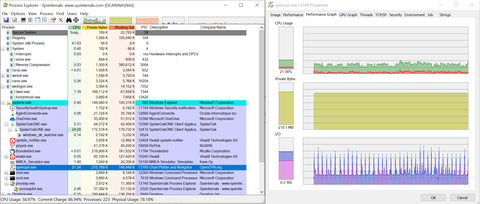
\includegraphics{2020-01-20_dgb_procexp_12_instrucjs_clients_alpha_01.png}
\href{img/2020-01-20_dgb_procexp_12_instrucjs_clients_alpha_01.png}{(zoom)}

    That is huge waste of the CPU power since the dials are not moving at
all. Let's make the following change in the script sending code and then
observe again:

\begin{verbatim}
        if ( m_istate == JSI_SHOWDATA ) {
            if ( m_data != m_lastdataout ) {
                wxString javascript =
                    wxString::Format(
                        L"%s%s%s",
                        "window.iface.newdata(",
                        m_data,
                        ");");
                RunScript( javascript );
                m_lastdataout = m_data;
            } // then do not load the system with the same script execution multiple times
        } // the instrument is ready for data
\end{verbatim}

    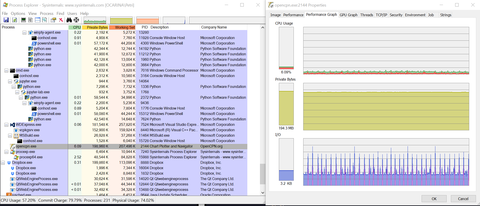
\includegraphics{2020-01-20_dgb_procexp_12_instrucjs_clients_alpha_02.png}
\href{img/2020-01-20_dgb_procexp_12_instrucjs_clients_alpha_02.png}{(zoom)}

    The CPU-load looks quite reasonable around 7 percent w/ i7 CPU and the
number of I/O operations is less than half of what it used to be!

    Of course, when one creates heavy oscillation in the r.p.m. values, for
example, the CPU load goes up, since the SVG-rendering of several dials
in this case is entering into the game - there is always a price to pay
for jumping dials! But it is noteworthy that the number of I/O
operations remain low, nevertheless.

    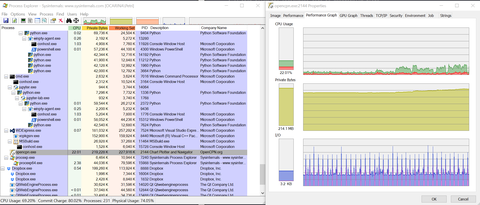
\includegraphics{2020-01-20_dgb_procexp_12_instrucjs_clients_alpha_02_cont_changes.png}
\href{img/2020-01-20_dgb_procexp_12_instrucjs_clients_alpha_02_cont_changes.png}{(zoom)}

    The background load can be further reduced by \textbf{randomizing the
threads} which are driving the JS instruments:

    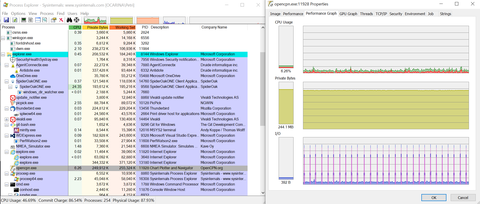
\includegraphics{2020-01-22_dgb_procexp_12_instrucjs_clients_alpha_02_randomized_threads.png}
\href{img/2020-01-22_dgb_procexp_12_instrucjs_clients_alpha_02_randomized_threads.png}{(zoom)}

    \hypertarget{overall-performance-in-hosting-systems}{%
\subsection{Overall performance in hosting
system(s)}\label{overall-performance-in-hosting-systems}}

    The paradigm of subscription of the JS instruments into the single
datasource which is provided by the \texttt{streamin-sk.cpp} is
efficient by the speed of tha call-backs and their little overhead. It
also limits the number of connections to the Signal K server node.

    The subscription paradigm probably (but not necessarily) needs to be
expanded to that steamer/parser itself. Starting from \emph{SignalK
server node v1.19.0} the subscription policy is made mandatory also for
the TCP socket data read. This can be used to our advantage regarding
the CPU load. The streamer is centralizing the data connection which is
good, but once we have set up of what we need to subscribe for, we could
reduce the CPU load of that streamer by asking it to subscribe only for
the values we are interested in.

    With NMEA Simulator we can reach quite considerable amount of messages,
which leads the \texttt{streamin-sk.cpp} thread to process about 290 -
300 floats per second resulting about 10 - 12 \% of constant CPU load
(Win20/i7), at the same time \texttt{npm} process, hosting the Signal K
server node has 7 - 8 \% CPU load.

    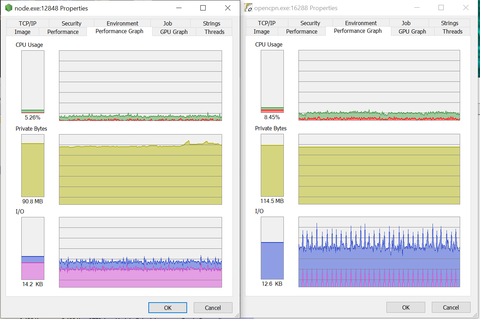
\includegraphics{2020-02-09_dgb_procexp_01_instrucjs_clients_alpha_02_sk1-21-0_max_nof_NMEA-2000_msgs.png}
\href{img/2020-02-09_dgb_procexp_01_instrucjs_clients_alpha_02_sk1-21-0_max_nof_NMEA-2000_msgs.png}{(zoom)}

    There is no doubt that the network distributed data producing and
consuming is a better configuration scheme: the Signal K server on a RPI
and the data consumer on another computer, like on Windows laptop or a
tablet. Here we make the other way around (because of the NMEA Simulator
being a Windows program) but it shows the idea of consuming one CPU core
on a RPI 4 for communication tasks:

    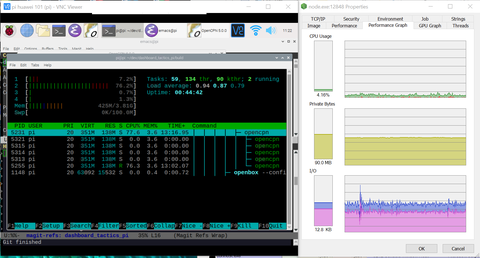
\includegraphics{2020-02-09_dgb_htop_procexp_01_instrujs_clients_alpha_02_sk1-21-0_RPIclient_WinSKsrv.png}
\href{img/2020-02-09_dgb_htop_procexp_01_instrujs_clients_alpha_02_sk1-21-0_RPIclient_WinSKsrv.png}{(zoom)}

    Resulting network traffic on the TCP port 8375, over WiFi:

    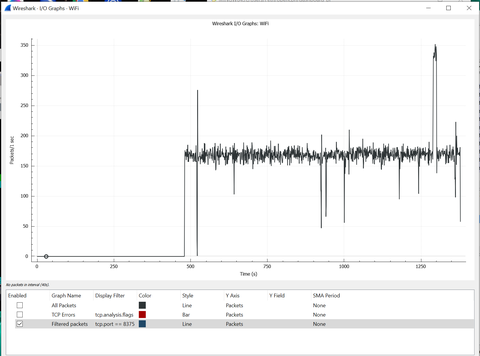
\includegraphics{2020-02-09_wireshark_wifi_rate_8375TCP_procexp_01_instrujs_clients_alpha_02_sk1-21-0_RPIclient_WinSKsrv.png}
\href{2020-02-09_wireshark_wifi_rate_8375TCP_procexp_01_instrujs_clients_alpha_02_sk1-21-0_RPIclient_WinSKsrv.png}{(zoom)}

    \hypertarget{help-my-fancy-application-looks-rotten-does-not-work-on-rpi}{%
\section{Help! My fancy application looks rotten / does not work on
RPI}\label{help-my-fancy-application-looks-rotten-does-not-work-on-rpi}}

    Let's consider our design constraints first: we are developing for
cross-platform, limited or old-fashioned web application run-time
support environment with very small screen or canvas area.

    Sounds familiar? Yes, it is like developing a HTML/CSS/JS application
for a telephone back in the day!

    You need to have the patience - and more importantly - the possibility
to carefully check and adjust at pixel level CSS files and debug
stubborningly failing JavaScript which worked fine on your browser.

    Unfortunately the \emph{iOS} or \emph{Android} USB-based development
tool connections to your \emph{Safari} or \emph{Chrome} will not be any
good in this case.

    There is, however a solution. It is not developed any more (since 2017)
but it still exists and \textbf{it still works}:
\href{https://people.apache.org/~pmuellr/weinre/docs/latest/}{WEINRE}.
Let's hope it is not going away, or that other tools for
\texttt{wxWidgets} \texttt{WebView} would emerge!

    \begin{quote}
\textbf{Attention vulnerabilities} - \emph{weinre} module has its
development stopped and it is as such a very vulnerable product. Use
\texttt{npm\ audit} to see the details of those. Make sure to use
--save-dev switch when installing to use it only for occasional
debugging during the development phase.
\end{quote}

    While waiting the new tools, I archived
\href{pdf/debugging_mobile_javascript_with_WEINRE_ibm_blog_2011.pdf}{this
paper}
(\href{https://www.ibm.com/developerworks/community/blogs/94e7fded-7162-445e-8ceb-97a2140866a9/entry/debugging_mobile_javascript_with_weinre?lang=en}{2011})
which nicely explains the remote portable device debugging concept and
what you can expect and what you cannot expect from WEINRE.

    \hypertarget{installating-weinre-on-rpi}{%
\subsection{Installating WEINRE on
RPI}\label{installating-weinre-on-rpi}}

    To use WEINRE, one needs to have web server. Luckily, on RPI this is
easy:

    Installing http-server on RPI

    If you are reading this, it is highly likely that you are using the
excellent
\href{https://github.com/SignalK/signalk-server-node/blob/master/raspberry_pi_installation.md}{SignalK
node server} on your RPI. That means that you have \texttt{node.js} and,
with it \texttt{npm} package manager.

    Install \href{https://www.npmjs.com/package/http-server}{http-server}
with command \texttt{sudo\ npm\ install\ http-server\ -g}.

    Using the command line, move to the directory where your application
file root is located and give command \texttt{http-server}. Leave it
running \emph{et voilà}, you have a web server!

    \hypertarget{get-weinre}{%
\subsubsection{Get WEINRE}\label{get-weinre}}

    \texttt{sudo\ npm\ intall\ -\/-save-dev\ weinre}

    \hypertarget{configuring-weinre}{%
\subsubsection{Configuring WEINRE}\label{configuring-weinre}}

    In your home folder, create a file
\texttt{\textasciitilde{}/.weinre/server.properties} with the following
contents:

    \begin{verbatim}
boundHost:    -all-
httpPort:     8081
reuseAddr:    true
readTimeout:  1
deathTimeout: 5
\end{verbatim}

    \hypertarget{launching-weinre-server}{%
\subsubsection{Launching WEINRE server}\label{launching-weinre-server}}

    Using (another shell) command line, type \texttt{weinre} and leave it
running.

    Now you should have two servers, \texttt{http-server} and
\texttt{weinre} running.

    \hypertarget{opening-the-weinre-debugger}{%
\subsubsection{Opening the WEINRE
debugger}\label{opening-the-weinre-debugger}}

    Start the RPI's browser, probably \emph{Chromium} (but I am using
\emph{Vivaldi}) and navigate to \texttt{localhost:8081}.

    The server's welcome page, \emph{weinre - web inspector remote} will
open. It will give you interesting information and even demos you may
want to try first opening them on a \textbf{separate} screen or tab.

    Likewise, you would open the debugger service,
\texttt{localhost:8081/client/\#anonymous} on a separate screen or tab.
This window is now waiting for a connection from your remote (or local)
\texttt{wxWidgets} \texttt{WebView} based application.

    \hypertarget{preparing-your-application-for-remote-debugging}{%
\subsubsection{Preparing your application for remote
debugging}\label{preparing-your-application-for-remote-debugging}}

    With ``\emph{remote}'' we understand your debug server running on the
Raspberry Pi, and either a \emph{webview} browser or OpenCPN with its
\texttt{WebView} class based instruments running on your Windows, Mac or
Linux development system

    Of course, it is not so ``\emph{remote}'' if the main debugging target
being the \emph{webview} browser or OpenCPN running on Raspberry Pi. But
since WEINRE access event those applications through the http-server, it
does not make any difference, in fact:

    One can have multiple hosts used at the same time, for testing and
debugging the same application on different run-time platforms.

    Each instance of the application must know where WEINRE server is
located. So you need to know your Raspberry Pi's IP-address in your
network. Let's say it is 192.168.8.103 : In really ``\emph{remote}''
test environments you would add the following line in your HTML:

    \begin{verbatim}
<!--script src="http://192.168.8.103:8081/target/target-script-min.js#anonymous"></script-->
\end{verbatim}

    It is not mandatory to use it in exclusively ``\emph{local}''
development, you can set:

    \begin{verbatim}
<!--script src="http://127.0.0.1:8081/target/target-script-min.js#anonymous"></script-->
\end{verbatim}

    Open the your application's HTML-file in \emph{webview} browser - drag
and drop works.

    As you can see above, this makes the application to download a
javascript module from the WEINRE server. It connects you the WEINRE
server's debug environment. If you not see the connection under the
\emph{Remote} tab, reload the page:

    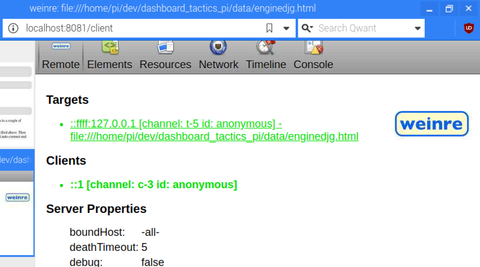
\includegraphics{2019-12-25_weinre_server_connected_to_local_host_client.png}
\href{pdf/2019-12-25_weinre_server_connected_to_local_host_client.png}{(zoom)}

    \hypertarget{debugging-with-weinre}{%
\subsubsection{Debugging with WEINRE}\label{debugging-with-weinre}}

    Please remember that this is \textbf{not} full blown JavaScript debugger
like the one which you can find from your browser. Before coming here
you have debugged your algorithms and you will use WEINRE only to find
and sort out the snagging incompatibility issues between the various
run-time environments.

    What can one do with WEINRE, then?

    \hypertarget{inspect-the-document-structure}{%
\subsubsection{Inspect the document
structure}\label{inspect-the-document-structure}}

    In the case of it is your JavaScript which dynamically constructs your
document structure contents, it would be a good omen for the rest of the
session if you can find actually the intended identifiers in the
structure:

    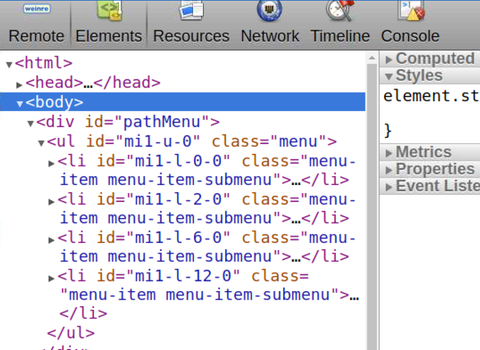
\includegraphics{2019-12-25_weinre_server_element_inspection.png}
\href{img/2019-12-25_weinre_server_element_inspection.png}{(zoom)}

    Like with the modern browsers, you can select a structure in the
``\emph{Elements}'' window and it will be highlighted in the
\emph{webview} browser, which is quite handy sometimes.

    ``\emph{Resources}'', ``\emph{Network}'' and ``\emph{Timeline}'' tabs
are quite useless and you should not expect to see anything interesting
there.

    ``\emph{Console}'', as the name implies allows you to inspect the
variables and show the \texttt{console.log()} output.

    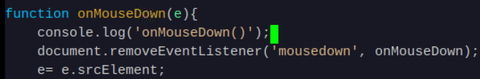
\includegraphics{2019-12-25_weinre_server_consolelog_code.png}
\href{img/2019-12-25_weinre_server_consolelog_code.png}{(zoom)}

    Finally, the answer to the question ``\emph{what to do?}'' if your
screen remains blank or if the mouse event does not work as you expect
is the following: Use the good old ``\emph{comment out suspicious code
blocks until your application loads}''-method!. Then put
\texttt{console.log()} calls in critical points.

    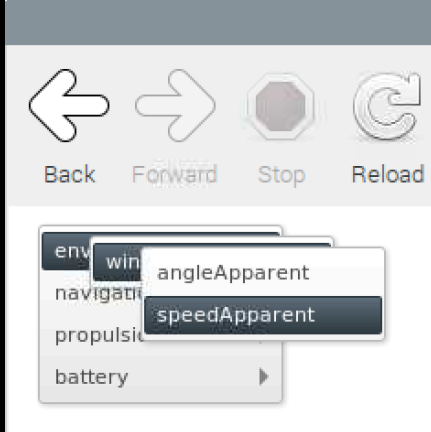
\includegraphics{2019-12-25_weinre_server_console_mouse_event.png}
\href{img/2019-12-25_weinre_server_console_mouse_event.png}{(zoom)}

    \begin{quote}
\textbf{NOTE} An older browser with developers tools is often enough to
resolve startup problems related to typos in variable names and such
(you do not need Weinre for that). Blow the dust out from your obsolete
Internet Explorer and hit key \textbf{F12}!
\end{quote}

    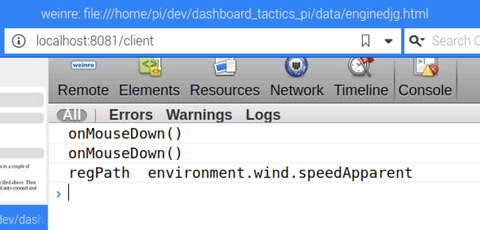
\includegraphics{2019-12-25_weinre_server_console_mouse_event_log.png}
\href{img/2019-12-25_weinre_server_console_mouse_event_log.png}{(zoom)}

    Rudimentary? Yes, but supposing that your algorithms are already tested
elsewhere, WEINRE allows you to have the necessary tools to avoid
guesswork based development!

    \hypertarget{debugging-data}{%
\section{Debugging Data}\label{debugging-data}}

    First of all, our interface is Signal K node server which puts out
Signal K. But it does not hurt to know how does it get the data from the
NMEA-2000 bus

    \begin{quote}
Since nobody can count the number of NMEA-2000 adaptations out there, we
use the excellent
\href{https://opencpn.org/wiki/dokuwiki/doku.php?id=opencpn:supplementary_software:signalk:a6\#how_to_use_a_nmea-simulator_to_stream_nmea-0183_and_nmea-2000_data}{NMEA-0183/2000
Simulator}
\end{quote}

    \hypertarget{nmea-2000-data-analysis}{%
\subsection{NMEA-2000 data analysis}\label{nmea-2000-data-analysis}}

    By far the easiest way is to use the log files provided by a proven
Signal K server node device support. It is unlikely that one will find a
bug here, but it is good practice to start the signal path debugging as
close to the source as possible.

    Turn on the log file usage for the connection, let the NMEA-2000 data
flow and check the result. You should find something like this:

    \begin{verbatim}
1580932802754;A;2020-02-05T20:00:02.735Z,2,127488,18,255,8,00,ac,0c,d6,02,02,ff,ff
1580932802758;A;2020-02-05T20:00:02.755Z,6,126996,18,255,134,14,05,9a,02,4e,4d,45,41,32,30,30,30,20,
73,69,6d,75,6c,61,74,6f,72,20,65,6e,67,69,6e,65,00,00,00,00,00,00,00,31,2e,
32,2e,30,2e,31,30,39,00,00,00,00,00,00,00,00,00,00,00,00,00,00,00,00,00,00,
00,00,00,00,00,31,2e,32,2e,30,2e,30,00,00,00,00,00,00,00,00,00,00,00,00,00,
00,00,00,00,00,00,00,00,00,00,00,00,32,30,39,37,31,34,37,00,00,00,00,00,00,
00,00,00,00,00,00,00,00,00,00,00,00,00,00,00,00,00,00,00,01,01
1580932802812;A;2020-02-05T20:00:02.811Z,6,60928,18,255,8,fb,ff,bf,ff,00,a0,64,c0
1580932802813;A;2020-02-05T20:00:02.812Z,2,127488,18,255,8,00,ac,0c,d6,02,02,ff,ff
1580932802813;A;2020-02-05T20:00:02.813Z,2,127488,18,255,8,00,ac,0c,d6,02,02,ff,ff
1580932802813;A;2020-02-05T20:00:02.813Z,2,127488,18,255,8,00,ac,0c,d6,02,02,ff,ff
1580932802814;A;2020-02-05T20:00:02.813Z,2,127488,18,255,8,00,ac,0c,d6,02,02,ff,ff
1580932802889;A;2020-02-05T20:00:02.814Z,2,127489,18,255,26,00,4c,0a,66,0e,5d,75,32,05,83,01,e1,d9,
a7,00,01,00,1f,00,ff,00,00,00,00,43,3d
1580932802889;A;2020-02-05T20:00:02.889Z,2,127488,18,255,8,00,ac,0c,d6,02,02,ff,ff
1580932802890;A;2020-02-05T20:00:02.889Z,2,127488,18,255,8,00,ac,0c,d6,02,02,ff,ff
...
\end{verbatim}

    The first line
\texttt{1580932802754;A;2020-02-05T20:00:02.735Z,2,127488,18,255,8,00,ac,0c,d6,02,02,ff,ff}
is 127488 Engine Parameters, Rapid Update

    From
\href{http://www.nmea.org/Assets/july\%202010\%20nmea2000_v1-301_app_b_pgn_field_list.pdf}{nmea2000\_v1-301\_app\_b\_pgn\_field\_list.pdf}

\begin{verbatim}
Field # Field Description
Provides data with a high update rate for a specific engine in a single frame message. The first field provides information as to
which engine.
1 Engine Instance
2 Engine Speed
3 Engine Boost Pressure
4 Engine tilt/trim
5 Reserved Bits
\end{verbatim}

See also (there are some contradictory information, probably vendor
dependencies!): *
\href{https://www.nmea.org/Assets/20090423\%20rtcm\%20white\%20paper\%20nmea\%202000.pdf}{NMEA2000-explained-white-paper.pdf}
* http://continuouswave.com/whaler/reference/PGN.html *
\href{http://data.over-blog-kiwi.com/0/54/01/67/20151122/ob_f92436_nmea2k-network-design-v2.pdf}{NMEA2K\_Network\_Design\_v2.pdf})
:

\begin{verbatim}
6.9 PGN 127488 – Engine Parameters, Rapid Update
Field 1: Engine Instance – This field indicates the particular engine for which this
data applies. A single engine will have an instance of 0. Engines in multi-engine
boats will be numbered starting at 0 at the bow of the boat incrementing to n going
in towards the stern of the boat. For engines at the same distance from the bow are
stern, the engines are numbered starting from the port side and proceeding towards
the starboard side.
2: Engine Speed – This field indicates the rotational speed of the engine in units of ¼
RPM.
3: Engine Boost Pressure – This field indicates the turbocharger boost pressure in
units of 100 Pa.
4: Engine tilt/trim – This field indicates the tilt or trim (positive or negative) of the
engine in units of 1 percent.
5: Reserved – This field is reserved by NMEA 
\end{verbatim}

    1: Engine instance = 00

    2: Engine speed: AC/0C = 0xCAC = 3244 . . . \(3244 \div 4 = 811 r.p.m.\)
(NMEA Simulator shows 811 OK)

    3: Engine Boost Pressure: D6/02 = 0x2D6 = 726 . . .
\(726*100Pa=72.6kPa\) (NMEA simulator was showing 72.6kPa at this moment
OK!)

    4: Engine Tilt/trim: 02 . . . \(2\%\) (NMEA simulator was showing
\(+2\%\) OK)

    Let's try with a negative value, with the simulator we set trim to
-24\(^{\circ}\)

    We read now:
1581197536148;A;2020-02-08T21:32:16.139Z,2,127488,18,255,8,00,60,12,d6,02,\textbf{e8},ff,ff

    e8 . . . 100 - e8 = 0x18 = 24

    \begin{quote}
Suspected anomaly in Signal K server node v1.21.0 conversion (maybe that
the driver is working correctly with intended hardware? In this case,
the hardware is screwed\ldots): \(\pm\) values are converted in Signal K
in an incoherent manner: like +2 becomes 2.0E-2 but -24 remains -12.0
and not -1.2E-1 as expected. I am fixing this in the subcscription
callback of \texttt{instrujs.cpp} now.
\end{quote}

    \hypertarget{sentence}{%
\subparagraph{127489-sentence}\label{sentence}}

    We read:
\texttt{1580932802889;A;2020-02-05T20:00:02.814Z,2,127489,18,255,26,00,4c,0a,66,0e,5d,75,32,05,\ 83,01,e1,d9,a7,00,01,00,1f,00,ff,00,00,00,00,43,3d}

\begin{verbatim}
6.10 PGN 127489 – Engine Parameters, Dynamic
Field 1: Engine Instance – This field indicates the particular engine for which this
\end{verbatim}

(see above, engine data is same)

\begin{verbatim}
2: Engine Oil Pressure – This field indicates the oil pressure of the engine in units of
100 Pa.
\end{verbatim}

4C/0A = 0xA4C = 2636 . . . \(2636 * 100Pa = 263.6kPa\) (NMEA simulator
was showing \(263.2kPa\) ? \(\equiv\) A48 . . . 48/0A ? also Instrujs
shows 264 kPa - looks like a rounding error!)

    \begin{verbatim}
3: Engine Oil Temperature – This field indicates the oil temperature of the engine in
units of 0.1°K.
\end{verbatim}

66/0E = 0xE66 = 3686 . . . \(368.6^{\circ}K \approx 95.6^{\circ}C\)
(NMEA simulator was showing \(95.6^{\circ}C\) = OK!)

    We read:
\texttt{1580932802889;A;2020-02-05T20:00:02.814Z,2,127489,18,255,26,00,4c,0a,66,0e,5d,75,32,05,\ 83,01,e1,d9,a7,00,01,00,1f,00,ff,00,00,00,00,43,3d}

\begin{verbatim}
4: Engine Temperature – This field indicates the temperature of the engine coolant in
units of 0.1°K.
\end{verbatim}

5D/75 = 0x755D = 30045 . . . \(300.45^{\circ}K \equiv 27.3^{\circ}C\)
(NMEA simulator was showing \(27.3^{\circ}C\) OK, so does the
\emph{instrujs})

Therefore : the units are \texttt{0.01°K} and \textbf{not}
\texttt{0.1°K}

    We read:
\texttt{1580932802889;A;2020-02-05T20:00:02.814Z,2,127489,18,255,26,00,4c,0a,66,0e,5d,75,32,05,\ 83,01,e1,d9,a7,00,01,00,1f,00,ff,00,00,00,00,43,3d}

\begin{verbatim}
5: Alternator Potential – This field indicates the alternator voltage in units of 0.01V. 
\end{verbatim}

32/05 = 0x532 = 1330 . . . \%13.3V\% (NMEA simulator was showing the
same OK).

    \begin{verbatim}
6: Fuel Rate – This field indicates the fuel consumption rate of the engine in units of
0.0001 cubic meters / hour.
\end{verbatim}

83/01 = 0x183 = 387 . . . \(387m^{3}/h * 0.0001 \equiv 38.7l/h\) which
is the value NMEA simulator is showing OK

    \begin{verbatim}
7: Total Engine Hours – This field indicates the cumulative runtime of the engine in
units of 1 second.
\end{verbatim}

We need to take another example than the rest what is discussed above
and below, since the hour counter is running all the time!

1581024474143;A;2020-02-06T21:27:54.141Z,2,127489,18,255,26,00,4c,0a,66,0e,5d,75,32,05,83,01,\textbf{59,3a,b0,00},01,00,1f,00,ff,00,00,00,00,43,3d

59 / 3a / b0 / 00 = 0x 00 b0 3a 59 = 11000289

\(11549273s \equiv 192487.88m \equiv 3208.13h\)

(NMEA simulator is showing 3213.8 hours right now, so the data is simply
a bit old, from the log file)

    We read:
\texttt{1580932802889;A;2020-02-05T20:00:02.814Z,2,127489,18,255,26,00,4c,0a,66,0e,5d,75,32,05,\ 83,01,e1,d9,a7,00,01,00,1f,00,ff,00,00,00,00,43,3d}

\begin{verbatim}
8: Engine Coolant Pressure – This field indicates the pressure of the engine coolant
in units of 100 Pa.
\end{verbatim}

01/00 = 0001 . . . 100Pa = 0.1kPa (NMEA simulator is showing exactly
this value OK)

    \begin{verbatim}
9: Fuel Pressure – This field indicates the pressure of the engine fuel in units of 1000
Pa.
\end{verbatim}

1F/00 = 0x001F = 31 . . . \(31*1000Pa\equiv31kPa\) (NMEA Simulator was
showing 30.7kPa OK)

    We read:
\texttt{1580932802889;A;2020-02-05T20:00:02.814Z,2,127489,18,255,26,00,4c,0a,66,0e,5d,75,32,05,\ 83,01,e1,d9,a7,00,01,00,1f,00,ff,00,00,00,00,43,3d}

\begin{verbatim}
13: Percent Engine Load – This field indicates the percent load of the engine in units
of 1 percent.
\end{verbatim}

43 = 67 . . . \(67\%\) (NMEA Simulator was showing 67\% OK)

    \begin{verbatim}
14: Percent Engine Torque – This field indicates the percent torque of the engine in
units of 1 percent. 
\end{verbatim}

3D = 61 . . . \(67\%\) (NMEA Simulator was showing 61\% OK)

    \hypertarget{debugging-using-python-can-and-serial-python}{%
\subsection{Debugging using Python CAN and Serial
Python}\label{debugging-using-python-can-and-serial-python}}

    There are as many alternatives for debugging NMEA-2000 bus - which is
essentially an enhanced CAN-bus - as there are adapters to connect into
it. You are welcome enhance this section with your knowledge about
those. Meanwhile, in order to have an idea how the NMEA-2000 device
support of Signal K server nodes sees the data, let's study a serial
line connected NMEA-2000

    \begin{verbatim}
import serial
ser = serial.Serial('COM30')
s = ser.read(100)
print(s)
\end{verbatim}

    One gets something like this:

\begin{verbatim}
b'\xf2\x01\xff\x12\x00\x00\x00\x00\x08\x00<\x08\xd6\x02\x02\xff\xff0\x10\x03
\x10\x02\x93%\x02\x01\xf2\x01\xff\x12\x00\x00\x00\x00\x1a\x00L\nf\x0e]u2\x05
\x83\x01\x10\x10\xb4\xb5\x00\x01\x00\x1f\x00\xff\x00\x00\x00\x00C=\xb8\x10
\x03\x10\x02\x93\x13\x02\x00\xf2\x01\xff\x12\x00\x00\x00\x00\x08\x00<\x08
\xd6\x02\x02\xff\xff0\x10\x03\x10\x02\x93\x91\x06\x14\xf0\x01\xff'
\end{verbatim}

Which is not that good, since one has both hex value and - when the
interpretation is possible - ASCII values mixed.

    This should, theoretically at least, work but does not show anything,
probaly because of the protocol differences between CAN and enhancing
NMEA-2000. We keep it here in case somebody has an idea how to get it
work.

\begin{verbatim}
import can

bus = can.interface.Bus(bustype='serial', channel='COM30', bitrate=115200)
for msg in bus:
    print(msg)
\end{verbatim}

    One can find attempts to print structured data without the aboev class,
but they are not apated to NMEA-2000:

    \begin{verbatim}
import serial
import struct

ser = serial.Serial('COM30')

fmt = "<IB3x8s"

while True:
   can_pkt = ser.read(16)
   can_id, length, data = struct.unpack(fmt, can_pkt)
   data = data[:length]
   print(data, can_id , can_pkt)
\end{verbatim}

    We get something like this:

\begin{verbatim}
b'\xff\x12' 328401424 b'\x10\x02\x93\x13\x02\x00\xf2\x01\xff\x12\x00\x00\x00\x00\x10\x02'
b'\x00\x00\x00\x00\x86\x14\x05\x9a' 335974803 b'\x93\x91\x06\x14\xf0\x01\xff\x12\x00\x00\x00\x00\x86\x14\x05\x9a'
b'0 simula' 1162694146 b'\x02NMEA2000 simula'
b'ne\x00\x00\x00\x00\x00\x00' 544370548 b'tor engine\x00\x00\x00\x00\x00\x00'
b'09\x00\x00\x00\x00\x00\x00' 841888000
...
\end{verbatim}

    \textbf{Pure hex is the best}, finally, one can search for \texttt{F201}
which is hex signature of PGN \texttt{127489}.

    \begin{verbatim}
import serial
import struct
import binascii

ser = serial.Serial('COM30')

while True:
   can_pkt = ser.read(4)
   print(binascii.hexlify(can_pkt))
\end{verbatim}

    Now, let's look from this data, for example, PGN 127489, Field, 3:
Engine Oil Temperature.

    b'10029325' b'0201\textbf{f201}' b'ff120000' b'00001a00'
b'4c0a\textbf{660e}' b'5d753205' b'8301802e' b'b8000100' b'1f00ff00'
b'00000043'

    Yes, it is still there, value 0x0e66 (see above for the interpretation).

    I reckon that now we can just trust the Signal K driver's author what
comes to the debug printing!

    \hypertarget{observing-the-data-coming-from-signal-k-server-node-delta-channel}{%
\subsection{Observing the data coming from Signal K server node delta
channel}\label{observing-the-data-coming-from-signal-k-server-node-delta-channel}}

    Starting from v1.19.0 the TCP delta channel requires also subscription
without exception. Good for the standard and overall charge of the
server but bad for debugging with an standard browser. One needs to be
able to send the subscription in non-human readable JSON-format and -
strangely - no headers are accepted before that, only the JSON
structure! That makes the usage of the developer tools a bit awkward in
the browser since how to compose such a message using the developer
tools?

    In case you manage to get the Signal K input streamer streaming
something (by default, it asks for everything), you can increase its
debug level in its JSON-configuration file \textbf{above reasonable}
(\emph{the thread will fail in its real-time parsing job because it
needs to interrupt its running to call for the log file writing from the
plugin process, also the log-file gets really quick really full, be
warned}):

    From \texttt{streamin-sk.cpp}:

\begin{verbatim}
if ( m_verbosity > 5 ) {
   m_threadMsg = wxString::Format(
      "dashboard_tactics_pi: Signal K type (%s) sentence (%s) talker (%s) "
       "src (%s) pgn (%d) timestamp (%s) path (%s) value (%f), valStr (%s)",
       type, sentence, talker, src, pgn, timestamp, path, value, valStr);
       wxQueueEvent( m_frame, event.Clone() );
} // then slowing down seriously with the indirect debug log
\end{verbatim}

    From \texttt{streamin-sk.json} (in data directory):

\begin{verbatim}
"streaminsk" : {
   "source"          : "localhost:8375", // not limited to localhost
   "api"             : "v1.19.0",        // version of Signal K server
   "connectionretry" : 5,                // [s] (min.=1s to reduce CPU load)
   "timestamps"      : "server",         // Signal K "server" or "local"
   "verbosity"       : 6                 //0=no,1=events,2=verbose,3+=debug
\end{verbatim}

    You will be well served:

    \begin{verbatim}
7:53:48 PM: dashboard_tactics_pi: DEBUG: Signal K JSON update server received delta-message:
{
   "context" : "vessels.urn:mrn:signalk:uuid:e5a702ea-0cb8-42cd-8f06-08c43bb5a4b6",
   "updates" : [
      {
         "source" : {
            "src" : "18",
            "label" : "Emu2000",
            "pgn" : 127489,
            "type" : "NMEA2000"
         },
         "$source" : "Emu2000.18",
         "timestamp" : "2020-02-08T18:53:47.921Z",
         "values" : [
            {
               "path" : "propulsion.port.temperature",
               "value" : 300.45
            }
         ]
      }
   ]
}

7:53:48 PM: dashboard_tactics_pi: Signal K type (NMEA2000) sentence () talker () src (18) pgn (127489) timestamp (2020-02-08T18:53:47.921Z) path (propulsion.port.temperature) value (300.450000), valStr (300.45)
\end{verbatim}

    \hypertarget{c-debugging-for-the-subscribed-value}{%
\subsection{C++ debugging for the subscribed
value}\label{c-debugging-for-the-subscribed-value}}

    \begin{quote}
The key point is to have only \textbf{one} \emph{instrujs} instrument
subcribed to data under inspection, in our example the
\texttt{propulsion.port.temperature} path. Please remind that we have
C++ object, subscription based data - it s getting pretty complex pretty
quickly from the debugging point of view!
\end{quote}

    With your (single) subcribed instrument active and working and hopefully
even showing some value, put your breakpoint here in
\texttt{instrujs.cpp}:

    \begin{verbatim}
void InstruJS::PushData(double data, wxString unit, long long timestamp)
{
    if ( !std::isnan(data) ) {
        setTimestamp( timestamp );  // Triggers also base class' watchdog
...        
\end{verbatim}

    Using the above, example debugging data, you should see the same value,
\emph{i.e.} 300.45.

    \hypertarget{javascript-data-debugging}{%
\subsection{Javascript data debugging}\label{javascript-data-debugging}}

    For performance reasons, \texttt{data.js} is not constantly printing
debug information to the \texttt{console.log()}. But nothing prevents
you to add such a statement in there. But since you will be running
within the OpenCPN, you would probably need to use \texttt{weinre}-tool
as discussed above to see the log output.

    Instead, I have used slow but more verbose method of using a browser and
its developer's tools. On can give the same commands through the
window.iface.* methods than the \texttt{instrujs.cpp} is doing (much
faster). With few such commands (with fake ID string but keep it always
the same, like \texttt{555-666} to profit the persistence), one can then
issue \texttt{iface.newdata()} commands.


    % Add a bibliography block to the postdoc
    
    
    
\end{document}
